{\setstretch{1.0} \textit{Manuscript in preparation.} \par}%Paper reference, note, other. Can remove. Single line space.
\section*{Abstract}
{\setstretch{1.0}  
Gastrointestinal side effects are the most common class of adverse reactions with orally absorbed drugs. They decrease the patient compliance to the treatment and reduce its efficacy. The prediction of the effects of a new chemical entity on the gut wall based on \textit{in vitro} data solely can improve the safety of marketed drugs and first-in-human trials. We used the drug-induced gene expression data from the connectivity map to build a drug-specific small intestine epithelial cell (sIEC) metabolic model. The combined measured \textit{in vitro} gene expression and the \textit{in silico} predicted metabolic rates in the gut wall were used as features for a multi-label support vector machine (SVM) to predict the occurrence of side effects. We showed that combining local gut wall specific metabolism with gene expression performs better than gene expression alone, which indicates the role of small intestine metabolism in the development of adverse reactions. Furthermore, we reclassified FDA-labelled drugs with respect to their genetic and metabolic profiles to show hidden similarities between seemingly different drugs. The linkage of xenobiotics to their transcriptomic and metabolic profile could take pharmacology far beyond the usual indication-based classification.
\par}%single line space

\newpage
\section{Introduction}
Side effects are unintended effects of administered xenobiotics that lead to the decrease of the efficacy of the treatment, a lower compliance of the patients, and eventually the cessation of the treatment with the development of adverse physiological consequences. Up to 25\% of drug development programs failed because of a lack of safety in first-in-human trials \cite{harrison2016phase}. Therefore, the prediction of side effects of drugs in the preclinical phase using solely \textit{in vitro} data holds the promise of decreasing the high attrition rates in drug development. Moreover, oral administration of drugs being the most common route of disposition, the gastrointestinal side effects are the most common class by occurrence \cite{bates1995incidence,makins2003gastrointestinal}, particularly in geriatry \cite{jain2009gastrointestinal}. Therefore, identifying compounds that can cause serious gastrointestinal adverse reactions from the ones that have benign effects could help optimizing the drug in the preclinical phase before the first-in-human trials.\\
The prediction of iatrogenic effects have been addressed mainly through a target-based approach, wherein the inhibition of a specific target could not only induce the desired effect but also suppresses all physiological process implicating the target protein \cite{campillos2008drug}. Recently, with the availability of genome-wide transcriptome profile of more than 20,000 compounds in the connectivity map \cite{subramanian2017next}, new approaches have considered linking the off-target effects to adverse reactions. Specifically, the interaction of the compound with non-target genes was hypothesized to drive the emergence of side effects. Recent efforts combined drug-induced gene expression with its chemical structure and Gene Ontology (GO) processes as features to accurately predict side effects \cite{wang2016drug}. Notably, it has been shown that metabolic genes are among the most predictive features for the classification \cite{wang2016drug}. Additionally, context-specific drug metabolic models built on generic reconstruction of human metabolism \cite{zielinski2015pharmacogenomic} allowed to identify metabolic dysregulation underlying the emergence of side effects.\\
In this study, we considered a context-specific metabolic model of gut wall where the drug-induced gene expression constrained the space of metabolic phenotypes. The uniform sampling of the solution space \cite{bordel2010sampling} allowed to derive differential scores between the drug specific model and the unperturbed model. Furthermore, we combined the metabolic reactions with drug-induced gene expression to build and cross-validate a multi-label support vector machine to predict the occurrence of side effects. Finally, the transcriptomic and metabolic profiles of drugs allowed to cluster compounds by their signatures enabling a new classification that goes beyond the usual drug indication, thereby offering new insights into drug repurposing.\\
The combination of local gut wall metabolism \cite{sahoo2013predicting} with drug transcriptomic profile allowed to contextualize gene expression data thereby increasing the predictive capability of side effect classifiers. Extending the classification to a more comprehensive set of side effect and tissue specific models could provide useful information at the preclinical phase of drug development thus reducing costs and attrition rates.

\section{Methods}
\subsection{Data generation}
We used the SIDER \cite{campillos2008drug,kuhn2010side} side effect database to extract intestinal side effect described as preferred terms (PT) in the MedDRA dictionary. The matching compounds were then queried in the L1000 LINCS dataset of compound gene expression\cite{subramanian2017next,lamb2006connectivity} through the iLINCS API \cite{keenan2017library}.  The level 4 data reporting the differential expression z-scores of the 978 landmark genes was subsequently subjected to the small intestine epithelial cell metabolic model (sIEC) \cite{sahoo2013predicting} which consists of 1282 metabolic reaction. On average 50 genes per drug model were mapped onto the sIEC. The exchange reactions for the sIEC model were set for standard European diet as described previously \cite{sahoo2013predicting} over 24h of interval. Consequently, we prioritized gene expression measured after 24h on intestinal cell lines, namely HT115, MDST8, SW-948, NCI-H716, HT-29, SW620, HCT 116, and LoVo. Only genes that were differentially expressed with a p-value lower than 0.05, were kept for further analyses. For each drug, an sIEC tailored metabolic model was generated in the form of a linear program (LP) (Section \ref{se:constraints}). Model infeasbilities arising from competing constraints, particularly with the exchange reactions were minimally relaxed both in cardinal and amplitude (Section \ref{se:constraints}), rendering them feasible. Under the drug constraints, we computed the possible flux values for each of the 1282 reactions through the uniform sampling of the linear program's solution space, using Artificially Centered Hit-and-Run (ACHR) implemented in the COBRA Toolbox \cite{heirendt2017creation}. The sampling was unbiased as it did not assume any objective function. We generated 100,000 points for each model using 1000 iteration step per point, starting from a 10,000 warmup points. Sampling of metabolic models allowed to determine a set of phenotypes of the modelled organism, particularly, it determines the distribution of reaction rates under a set of constraints \cite{bordel2010sampling}. For each metabolic reaction of a specific drug-constrained sIEC, the sampled flux distribution was compared to the drug-free sIEC model and z-scores were derived for each reaction.
Using the generated data, we created a matrix consisting of gene expression and metabolic flux in columns representing the features, and drugs in rows representing the observations. The matrix had 605 drugs and 2260 features consisting of 978 landmark genes and 1282 metabolic reactions, with standardized predictors as z-scores that were directly used for learning and cross-validation. 
We computed the minimal and maximal flux capacity for each reaction using Flux Variability Analysis (FVA) and used them as features in the classification as suggested previously \cite{shaked2016metabolic}. In this case the feature matrix had 1282*2 columns. We also considered the gene expression matrix alone with 978 genes corresponding to the columns.
\subsection{Subjecting gene expression as constraints on metabolic models} \label{se:constraints}
A manually curated metabolic model of the small intestine epithelial cell (sIEC) was previously constructed to study the effect of inborn errors of metabolism (IEMs) on human physiology \cite{sahoo2013predicting}. The metabolic model is formulated as a linear program as follows:
\begin{alignat}{2} 
  & \text{max: } &  & c^{T}v
  \label{se:eq1}\\
  & \text{subject to: } &  &  \nonumber
                \begin{aligned}[t] \\
                & Sv=0 \\
                & v_{min} \leq v  \leq  v_{max}
                \end{aligned}
  \nonumber
\end{alignat}
,where $c^{T}.v$ is the objective function, $v$ is the flux vector of metabolic reactions, $c$ is the vector of objective coefficients, $S_{(m,n)}$ is the stoichiometric matrix linking $m$ metabolites and $n$ reactions, $v_{min}$ is the reaction lower bound vector, and $v_{max}$ is the reaction upper bound vector. The system assumes steady state such that $S.v=0$, which is referred to as Flux Balance Analysis (FBA)\cite{orth2010flux} . Flux variability analysis (FVA) \cite{mahadevan2003effects} determines the minimal and maximal value feasible by each reaction, through maximizing and minimizing for each reaction as an objective function, consistent with the applied constraints.
Differential gene expression $z_i$ of gene $i$ encoding reaction $j$ modifies the allowable range of each reaction obtained by FVA such as the following:
\begin{equation*}
\begin{gathered}
v_{min,j}=min_{FVA,j}+z_i*std(v_j)\\
v_{max,j}=max_{FVA,j}+z_i*std(v_j)
\end{gathered}
\end{equation*}
,where $v_{min}$ and $v_{max}$ are the new lower and upper bounds of the sIEC drug model, and $min_{FVA}$ and $max_{FVA}$ are the lower and upper bounds of the drug-free sIEC determined by FVA, $std(v_j)$ is the standard deviation in reaction $j$ assuming a normal distribution of the fluxes between $min_{FVA}$ and $max_{FVA}$.
Similar to E-Flux \cite{colijn2009interpreting,brandes2012inferring}, this formulation of reaction constraints allows to keep the original structure of the model and changes the reaction bounds according to gene expression, because transcript levels cannot be used as conclusive evidence about the enzymatic activity of proteins \cite{machado2014systematic,kosti2016cross,franks2017post} and metabolic fluxes but are rather used to constrain the capacity and the space of possible flux values of the corresponding reaction. Because FVA bounds determine the solution space, scaling FVA bounds by gene expression constrains the sampling in a new space. Other recent formulations considered protein concentration to constrain flux capacity \cite{sanchez2017improving}.\\
Infeasible sIEC-drug model may occur because of conflicting constraints. If problem \ref{se:eq1} is infeasible, we minimally relaxed the constraints in both the amplitude of relaxation and the cardinal of relaxed reactions, through solving the following problem:
\begin{alignat*}{2} 
  & \text{min: } &  & ||p||_{1},||q||_{1}\\
  & \text{subject to: } &  &  
                \begin{aligned}[t] \\
                & Sv=0 \\
                & v_{min} - p \leq v  \leq  v_{max} + q
                \end{aligned}
\end{alignat*}
,where $p$ is the relaxation vector of the lower bound and $q$ is the relaxation vector of the upper bound. Minimizing the 1-norm of $p$ and $q$ ensures both sparsity (minimal cardinal of reactions to be relaxed), with minimal total sum of relaxation amplitude.
\subsection{Building the multi-class support vector machine}
The support vector machine multi-label learning was converted to 43 binary SVM single-label problems, using binary relevance in a one-versus-all scheme, where each classifier corresponded to an intestinal side effect as reported by SIDER preferred terms. The side effects occurring for only one drug were discarded and the total set was reduced to 36 side effects. The dataset used in classification were standardized in the SVM call.\\
The support vector machine classifier \cite{cristianini2000introduction} was compared to a set of classifiers namely, Random forest \cite{breiman2001random}, Logistic regression \cite{mccullagh1984generalized}, and Na\"{i}ve Bayes \cite{friedman2001elements} with their defaults parameters (Figure \ref{fig:s1algo}). The performance was assessed using the following metrics \cite{baldi2000assessing}: accuracy, area under the ROC curve (AUROC), area under the precision-recall curve (AUPR), weighted accuracy, and weighted recall. The weighted recall and weighted accuracy were computed using the average of the accuracy and recall of each label, weighted by the label size.
\subsubsection{Feature selection algorithm}
Given the high number of features, we proceeded to the selection of the most predictive genes and metabolic reactions through various algorithms using the feature selection toolbox \cite{RoffoICCV17} implemented in MATLAB (2017a release, Natick, MA, USA). The genes and metabolic reactions were then ranked by importance and used as input for the SVM multi-label model.
We tested 11 method of feature selection and compared them with regards to the performance of the SVM classifier as assessed by the area under the ROC curve (Figure \ref{fig:s1seff}).  The algorithms tested with their default parameters were ReliefF \cite{kira1992feature}, mutinffs \cite{luo2011methods}, FSV \cite{bradley1998feature}, Laplacian \cite{he2006laplacian}, MCFS \cite{cai2010unsupervised}, L0 \cite{han20150}, Fisher score \cite{gu2012generalized}, udfs \cite{yang2011l2}, llcfs, cfs \cite{hall1999correlation}.
ReliefF showed the highest predictive capability for the selected features and was kept for further analysis. Briefly, the algorithm ranks the features by importance based on a k-nearest neighbour graph. Consequently, the k parameter has to be optimized.
\subsubsection{k parameter of ReliefF}
The k parameter of ReliefF was varied through a range of values and the results were compared with respect to the area under the ROC curve. Usually a low value of k would not allow for strong separation of predictive features, while a k equal to the number of drugs would lead to the failure of the algorithm. A k equal to 80 allowed to obtain the highest predictability of the model (Figure \ref{fig:s2seff}).
\subsubsection{Number of features}
The number of the most predictive features was assessed through testing different values. The ReliefF algorithm takes as input the feature matrix and the corresponding side effect labels of the training set and computes the ranking and weights of the features. Selecting 20 features allowed to obtain the highest area under the ROC curve (Figure \ref{fig:s3seff}).
\subsubsection{Cross-validation method}
In order to avoid over-fitting and to enhance the accuracy of the classifier, various cross-validation methods were tested. K-folds cross-validation consists of splitting the dataset into k parts and performing learning on k-1 folds and the last fold would be used for testing. The leave-one-out cross-validation trains the classifier on n-1 points and validates the prediction on the n\textsuperscript{th} data point. The 3, 5, and 10 fold cross-validation as well as leave-one-out were compared for loss and predictability (\nameref{S5_Fig}). As cross-validation methods seemed comparable in prediction outcome (\nameref{S5_Fig}), we selected 3-fold cross-validation for further analysis because it requires less computation time. The process is summarized in the following steps:
\begin{enumerate}
\item	Divide the dataset into test (20\%) and training (80\%) set	
\item	Train a single-label classifier for each label with 3-fold cross-validation on the training set
\item	Repeat step two twice with a different partition of the training and validation set
\item	Predict the label of the test set using the trained models
\item	Repeat step one to four, 100 times taking each time a different partition of the test and training set.
\end{enumerate}
Finally, the posterior probabilities and the prediction loss on the test set were averaged for each side effect label.
\subsubsection{Misclassification cost}
Class imbalance is frequently encountered in biological datasets \cite{sontrop2011evaluation,haque2014imbalanced}. In our case, the occurrence of intestinal side effects varies widely from frequent unspecific disorders to rare side effects occurring with a few drugs. The misclassification cost matrix $C$ was set to the inverse of the label frequencies such that:\\
\begin{center}
$ C=
\begin{pmatrix} 
0 & \frac{1}{n_t-S_f} \\
\frac{1}{S_f} & 0 
\end{pmatrix}
$
\end{center}
, where the rows correspond to the observed labels, the columns correspond to the predicted labels in each binary classifier, $n_t$ is the size of the training set, and $S_f$ the side effect frequency. The effect of class balance (Figure \ref{fig:s5seff}) improved the classification performance.
\subsubsection{Observation weight}
Intestinal side effects occur with different empirical frequencies per drug. For every label, the weight of every drug was set to its frequency as reported in the SIDER database. Information about 485 side effect frequency were available over 1053 total number of side effects induced in the 36 labels. The missing information was set to the default of 1 and no further data imputation was done. Adding observation weights induced a slight decrease in the mean of the area under the ROC curve for intestinal side effects (Figure \ref{fig:s6seff}) and was not subsequently kept as a parameter in the model, likely because of the effect of the missing 54\% of side effect frequency.
\subsubsection{SVM kernel}
The kernel functions of support vector machines that were tested include a linear, Gaussian and 3\textsuperscript{rd} order polynomial function. The Gaussian kernel function had the highest mean of the area under the ROC curve per label (Figure \ref{fig:s7seff}) and was consequently set as a label-wide function. We also looked for the optimal kernel functions per label using MATLAB hyperparameter optimisation routine.
\subsubsection{Optimal hyperparameters}
The optimal hyperparameters obtained for the SVM in the previous analyses and summarized in table \ref{tbl:tbls1ch2} ensured high predictability and accuracy. Additionally, the automatic tuning of hyperparameters available in MATLAB was tested for hyperparameters listed in table \ref{tbl:tbls2ch2}. The automatic tuning routine finds the optimal set of parameters that minimize the cross-validation loss, where each binary classifier can have a different set of optimal parameters. Manually tuning global hyperparameters had a better area under the ROC curve than individually optimized hyperparameters (Figure \ref{fig:s8seff}) because the set of automatically tuned parameters in the 2017a release of MATLAB does not include all of the parameters, particularly the number of features and the feature selection method.
\subsection{Drug community identification, validation, and interpretation}
\subsubsection{Graph clustering}
A significance test on the principal components was performed using a 100 independent permutation of the columns of the feature matrix. 15 principal components had a p-value < 0.001 and were retained for subsequent analysis. Then we constructed a graph based on the k-nearest-neighbour (KNN) \cite{altman1992introduction} of each drug with k equal to 20, using the Jaccard index as a distance metric.
\begin{equation*}
J(d_A,d_B )=\frac{|d_A \cap d_B |}{|d_A \cup d_B |}
\end{equation*}
, where $d_A$ and $d_B$ are two given drugs in the networks, $|d_A \cap d_B |$ is the number of common neighbours and $|d_A \cup d_B |$ is the union of drug neighbours.
\subsubsection{Community detection}
Drug clusters in the network were identified using the Jaccard-Louvain algorithm \cite{blondel2008fast} as previously reported \cite{shekhar2016comprehensive} and the second level of community clustering gave eight clusters and was selected for further analysis. 
\subsubsection{Cluster visualisation}
For further validation and visual inspection, the clusters were visualized using the Barnes-Hut Stochastic Neighbourhood Embedding (Bh-SNE) \cite{van2013barnes}, with Euclidean distance, a perplexity of 30 and exaggeration of 4 on the 15 first principal components of the combined feature matrix. The seed used for the plot was 97.
\subsubsection{Cluster validation}
We performed network perturbations to assess the stability of the identified clusters. The value of k in the KNN algorithm was randomly selected in a uniform distribution between 2 and 50. We then selected independently 85\% of the drugs and built the Jaccard-based adjacency matrix, of which we removed 5\% of the edges and added 5\% of new random edges. Finally random noise values were added to the edges and the Jaccard-Louvain\cite{blondel2008fast} algorithm identified communities in the perturbed network. The process was repeated 200 times.
To validate the selected clusters \cite{shekhar2016comprehensive}, stability and purity were selected as external measures and were computed for each cluster \cite{von2010clustering}. Stability is measure of diversity in the clusters of each perturbation trial. Briefly, if the points assigned to a given cluster in a given trial have a high diversity of points from the original clustering assignment, the stability would be low. Stability was computed as the following:
\begin{gather*}
\begin{cases}
  Stability=1-instability\\
  Instability=\frac{1}{n} \sum_{i=1}^{n} \frac{E_{i}}{E_{i}^{Tot}}\\
  E_i=\sum_{i} p_{i}log(p_i)\\
  E_{i}^{Tot}=\sum_{j=1}^{m}p_{j}E_{j}
\end{cases}
\end{gather*}
, where $E_i$ is the entropy of a given cluster in trial $i$, $E_i^{Tot}$ is the total entropy in trial $i$, $p_i$ is the fraction of a given cluster size over all data points in trial $i$, $m$ is the number of clusters and $n$ is number of trials.
Purity is similar to stability and consists of the enumeration of data points in a given cluster $i$ that were labelled as cluster $j$. Purity is computed as follows:
\begin{gather*}
\begin{cases}
  Purity=1-\sum_{j=1}^{m} \frac{|cl_{j}|}{|nDrugs|}P_{j}\\
  P_{j}=\frac{1}{|cl_{j}|}Max_{i}(|cl_{j}^{i}|)
\end{cases}
\end{gather*}
, where $m$ is the number of clusters, $|cl_j|$ is the size of cluster $j$, $P_j$ is the purity of cluster $j$, $Max_i(|cl_{j}^{i} |)$ is the size of the largest cluster $i$ contained in cluster $j$ of the unperturbed clustering.
\subsubsection{Gene set enrichment}
In each cluster, the top differentially expressed genes were identified and submitted for pathway enrichment in KEGG \cite{kanehisa2017kegg} through Enrichr API \cite{kuleshov2016enrichr,chen2013enrichr}. Then the 10 most significantly enriched terms $(p<0.05)$ were assigned to each cluster.
\section{Results}
The prediction of iatrogenic gastrointestinal drug effects based on \textit{in vitro} data could improve the assessment of safety of new chemical entities. We combined drug-induced gene expression data with metabolic models of the gut wall to develop an SVM classifier. We employed the classifier to predict the occurrence of common gastrointestinal side effects and the biological processes involved in their development. Furthermore, we classified the drugs using their transcriptomic and metabolic signatures to provide insights into drug action and mechanism. Finally, including more tissues through context-specific metabolic models could extend the approach to additional labels of side effects.
\subsection{Generating the combined drug gene expression and metabolism matrix}
\begin{figure}[!ht]
\centering
	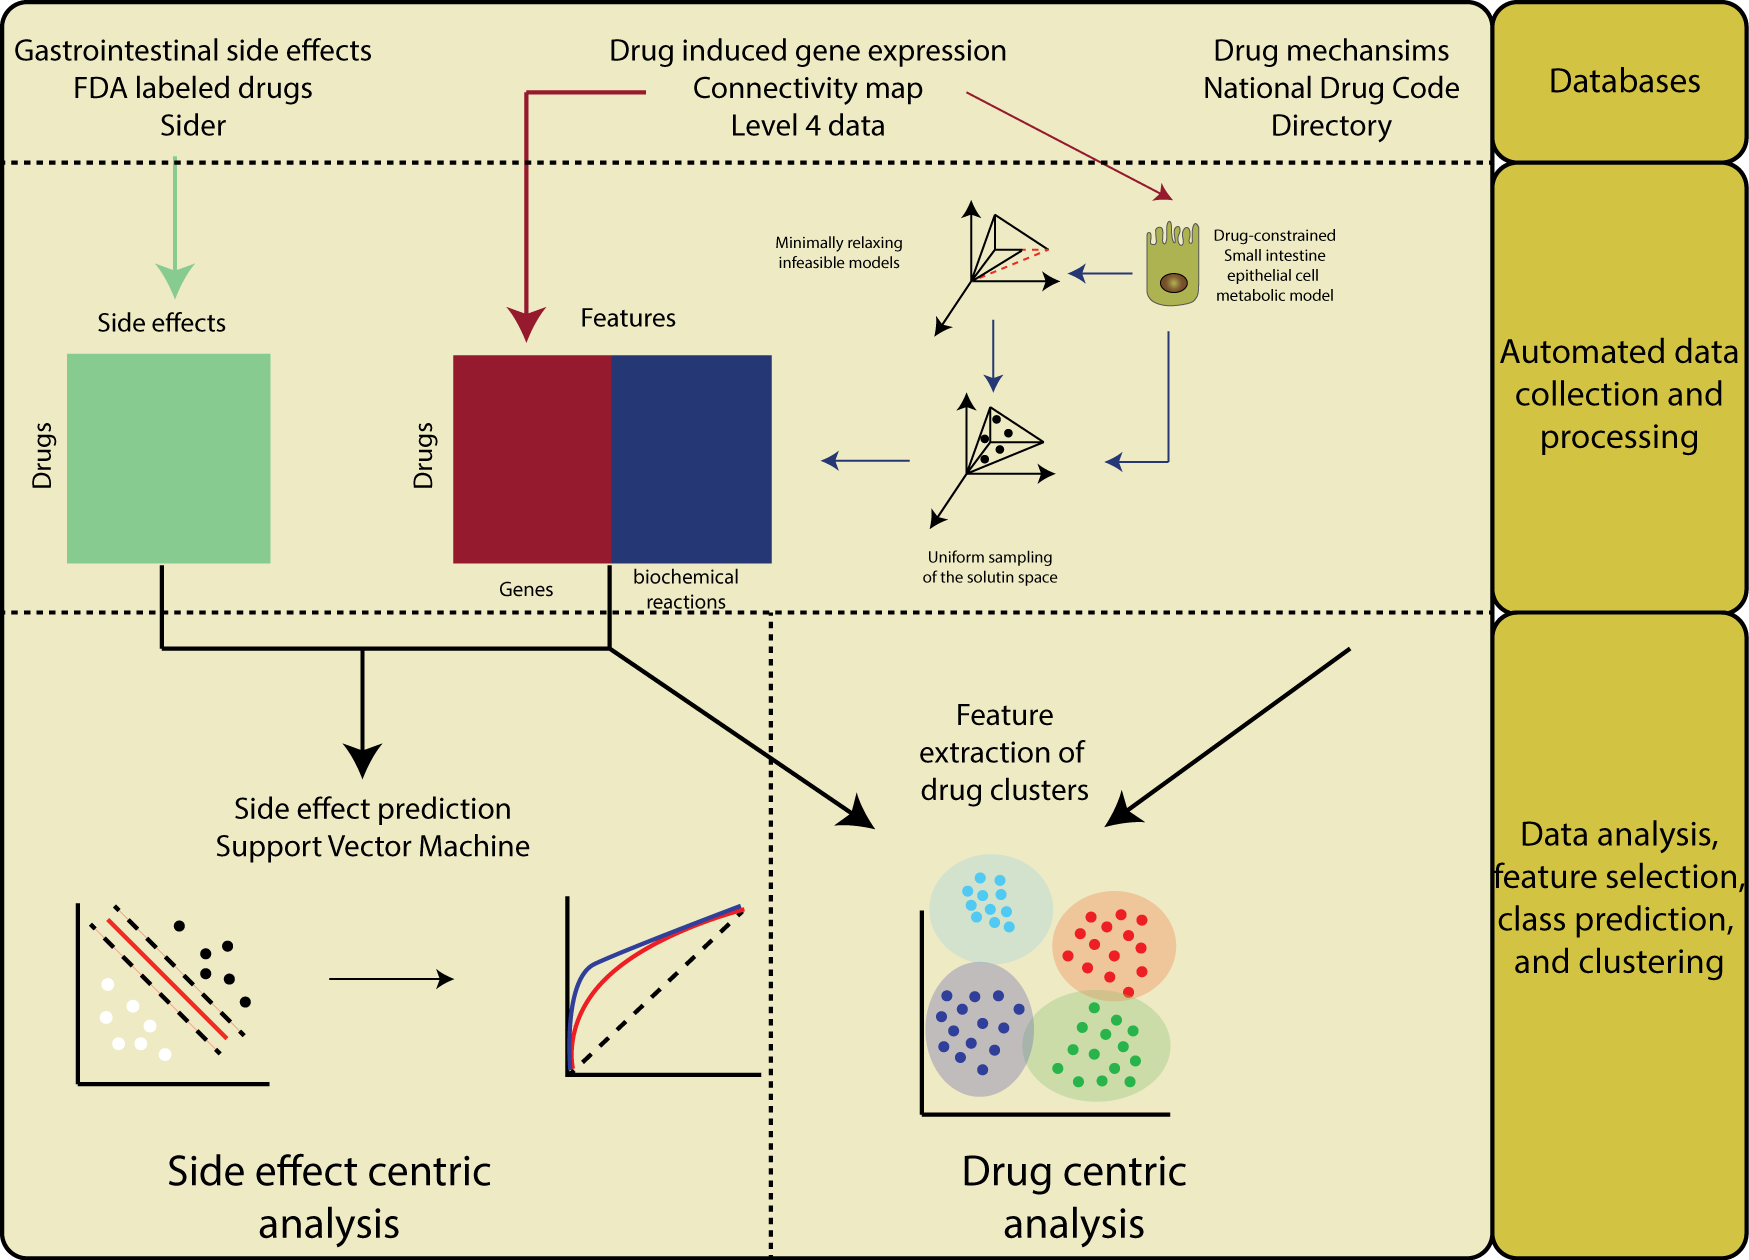
\includegraphics[width=\textwidth,height=\textheight,keepaspectratio]{sideEffects/Figure1.png}%Figure from images\Figure1.png
	\caption[Overview of the automatic data collection pipeline.]{Overview of the pipeline of data generation and analysis in this study. Drug induced gene expression were collected through the connectivity map API. The drug side effects occurrence was obtained from the SIDER database, and the drug mechanism and physiological effect was collected from the FDA National Drug Code Directory (NDCD). The drug-induced gene expression were subjected as constraints on a small intestine epithelial cell (sIEC) metabolic model to derive a context-specific model for each drug. After minimally resolving infeasible models, the uniform sampling of the solution space of the sIEC allowed to derive z-scores of metabolic fluxes in the treated and drug-free model. Combining the drug-induced gene expression with predicted differential metabolic fluxes in a single matrix allowed to train and cross-validate a multi-label support vector machine. Finally, the clustering of drugs based on their transcriptomic and metabolic profiles allowed to find hidden similarities beyond the indication based-classification.}
	\label{fig:seff1}
\end{figure}
In order to model drug effects on the gastrointestinal system, a manually-curated constraint-based model of the small intestinal epithelial cell (sIEC) \cite{sahoo2013predicting} was contextualized for each drug. The upper and lower bounds of every metabolic reaction were adjusted by the relative expression of the gene encoding the enzyme catalysing the reaction. The obtained context-specific drug-sIEC model was generated for every drug using the differential gene expression data obtained from the connectivity map \cite{subramanian2017next}. In models where the subjected constraints rendered the linear program infeasible, a set of reactions of minimal cardinality was relaxed by a minimal amplitude to obtain a feasible model. In order to assess the impact of drug constraints on metabolic models, the minimal and maximal metabolic flux per reaction was computed by FVA for each drug-constrained sIEC as suggested previously \cite{shaked2016metabolic}. Although, informing the classifier of the distribution of possible flux values per reaction rather than its bound could be of higher predictive capability. We sampled the drug-constrained solution space of each sIEC model and derived differential scores between the flux distribution per reaction of the drug-free sIEC and the drug-constrained sIEC. Following these steps, we obtained four features matrices: the differential gene expression of each drug obtained from the connectivity map, the FVA metabolism matrix obtained by the upper and lower bound of each reaction, the sampling metabolism matrix consisting of the differential score of flux value distribution per reaction, and the combined gene expression and sampled metabolism matrix which is a combination of the first and third matrices. The class matrix relating each drug to its side effects was obtained through parsing the SIDER database \cite{kuhn2015sider}. Further information about drug mechanisms, physiological effect, marketing date, and pharmacological class were obtained from the FDA NDCD database (Figure \ref{fig:seff1}).
\subsection{Combining measured gene expression and simulated gut wall metabolism predicts intestinal iatrogenic effects}
Drug induced gene expression provided strong features for side effect prediction, especially with side effect classes that have links to metabolism \cite{wang2016drug}. We used this finding to further improve the prediction of intestinal side effects through subjecting gene expression as constraints in the metabolic model of small intestine epithelial cell (sIEC), thereby contextualizing gut wall metabolism to derive the intestinal metabolic fingerprint of every drug. As previously observed \cite{wang2016drug}, gene expression alone was the support of most predictive features (Figure \ref{fig:seff2}-A). Metabolic reaction fluxes alone were less predictive as it takes into account the genes with metabolic activity in the sIEC (Figure \ref{fig:seff2}-A). Particularly, sampling the metabolic model allowed to improve the classification as it informs about the distribution of metabolic fluxes per reaction rather than the minimal and maximal bound of metabolic reactions alone as reported by FVA (Figure \ref{fig:seff2}-A). Combining gene expression and predicted metabolism gave the highest predictive rates in the multi-label SVM classifier as average of individual labels (Figure \ref{fig:seff2}-A), and in comparison to other classifiers (Figure \ref{fig:s1algo}).\\
Unspecific or likely non metabolic side effects such as gastrointestinal obstruction were among the least predictable with an area under the ROC curve of 0.67 using combined gene expression and sampled reaction fluxes. Side effects involving gut wall metabolism were highly predictable using combined features (Figure \ref{fig:seff3}, Table \ref{tbl:tbls3ch2}) such as intestinal carcinoma (0.96), ulcer (0.97), and toxicity (0.92). The merged intestinal side effect classifier using the individual binary classifiers could better predict (0.94) intestinal side effects based on combined gene expression and metabolism in comparison to gene expression (0.935)  or metabolism alone using FVA (0.92) and sampling (0.931) as shown by the micro-averaged ROC curve (Figure \ref{fig:seff2}-B). The most predictive metabolic reactions were enriched in the subsystems of sIEC and the most predictive genetic features were enriched in gene ontology biological processes database (both at p<0.001). The 10 most represented subsystems mainly involved transport in various locations (extracellular, exchange, mitochondrial, endoplasmic reticulum)  as well as catabolic and synthetic functionalities (Figure \ref{fig:seff2}-C). The gene ontology biological processes enriched groups involved mainly the regulation of transcription and apoptotic process (Figure \ref{fig:seff2}-D).  
\subsection{Drug  classification  using transcriptional and intestinal metabolic activity}
\begin{figure}[!ht]
\centering
	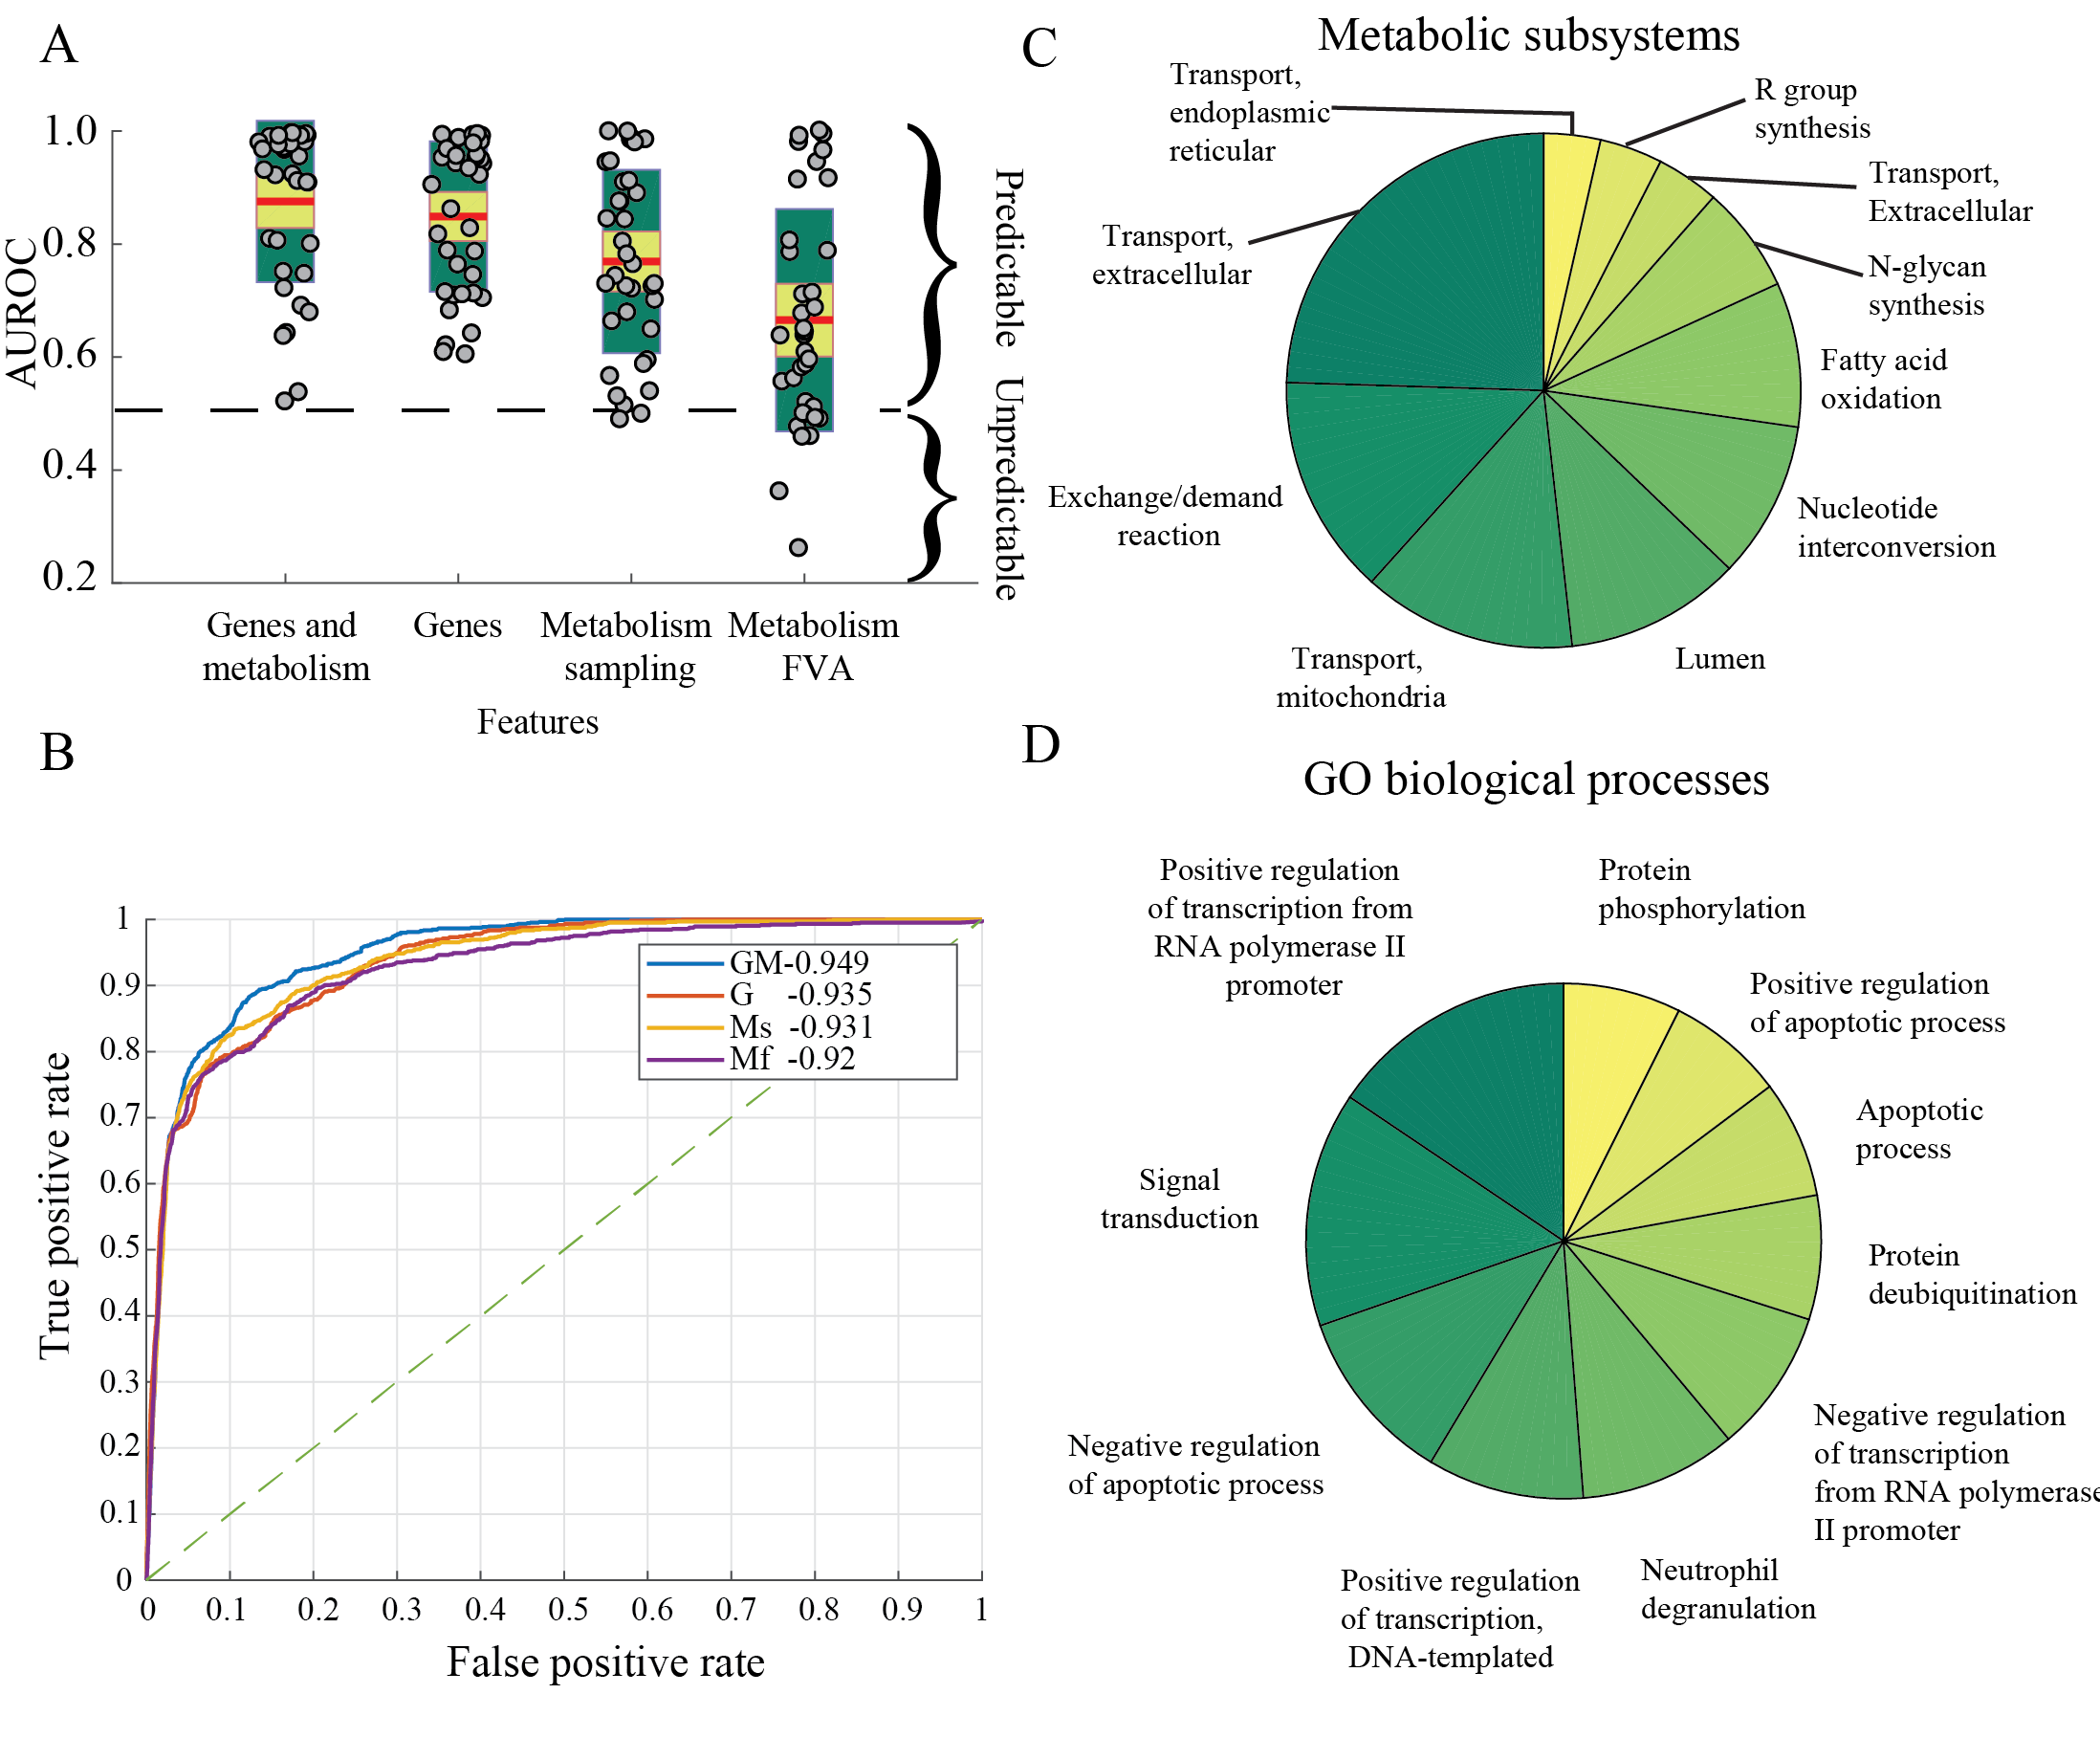
\includegraphics[width=\textwidth,height=\textheight,keepaspectratio]{sideEffects/Figure2.png}%Figure from images\Figure1.png
	\caption[Prediction performance of the multi-label SVM.]{Evaluation metrics for the multi-label support vector machine intestinal side effects classifier. A-Comparison of individual side effect classifier predictive capability as measured by the out-of-sample area under the ROC curve using genetic, metabolic, and combined genetic and metabolic features. B-ROC curve of the micro-averaged multi-label SVM classifier using genes, metabolism and combined genes and metabolism as features. C-Top 10 enriched metabolic subsystems and D-gene ontology biological process terms ranked by the number of metabolic and genetic representatives. G stands for genes, Ms for metabolism sampling, Mf for metabolism FVA, and GMs for genes and metabolism sampling.}
	\label{fig:seff2}
\end{figure}
\noindent The construction of the drug feature matrix consisting of gene and metabolic reaction vectors per drug allowed the use of clustering techniques to classify drugs in the gene and metabolism space. Using the community detection algorithm Jaccard-Louvain \cite{blondel2008fast}, we identified eight drug clusters based on their genetic and metabolic signature (Figure \ref{fig:seff4}-A). Each cluster had a stability and purity greater than 0.75 (Figure \ref{fig:s9seff}-D). In particular, transcriptional and intestinal metabolic activity were aligned with the identified clusters (Figure \ref{fig:seff4}-B). Interestingly, the identified clusters did not map on the FDA NDCD’s Established Pharmacological Class (EPC) (Figure \ref{fig:s9seff}-A) suggesting that classical indication-based classification could overlook genetic and molecular aspects of small molecules' pharmacodynamics. Most small molecules had a low genetic and  metabolic fingerprint as reported previously \cite{kuleshov2016enrichr} and targeted mainly the various transport subsystems (Figure \ref{fig:s9seff}-C) of the enterocyte, which is the main function of the gut wall. Cluster one and eight involved a high number of genes and metabolic reactions mainly due to cytotoxic drugs which was also reflected on the FDA NDCD’s Physiological Effect (PE) (Figure \ref{fig:seff4}-C) by the presence of terms linked to inflammation and immunity. Additionally, cluster eight and one were linked to malignant side effects (Figure \ref{fig:s9seff}-A).\\
Cluster seven had a high number of active fluxes in the small intestine epithelial cell. Interestingly, a number of terms linked to the central nervous systems were found, which hints to potential gut-brain shared molecular processes, probably linked to the similar composition of the blood brain barrier and the gut wall transporters \cite{banks2008blood}. In addition to cluster seven, cluster two had a low transcriptomic and a high metabolic profile. The EPCs linked to these clusters were mostly compounds whose action is mediated through metabolic, e.g., xanthine oxidase, or signalling, e.g., PPAR$\alpha$ molecule binding (Figure \ref{fig:seff4}-D). Ubiquitous targets, e.g., cyclooxygenase and histamine receptors would consequentially induce pronounced metabolic effects.\\
On the high transcription and high metabolism profile represented by cluster one and eight (Figure \ref{fig:seff4}-E), the presence of molecules acting on the central nervous systems by their FDA NDCD’s Mechanism of Action (MoA) confirms links between the gut and brain metabolism. Additionally, since cluster one and eight encompassed anticancer drugs as previously observed, this finding further supports ongoing repurposing trials of antidepressants in cancer therapy \cite{jahchan2013drug}. 
Moreover, neurokinin-1 antagonists, a class of drugs prescribed for the suppression of cytotoxic drug-induced emesis, and 5-lipoxygenase inhibitors, indicated for inflammatory bowel disease, had a high genetic and metabolic profile indicating potential links between gut symptomatology and genome-wide transcriptional and metabolic modulation. 
%Expectedly, antibiotics were among cluster one and cluster eight. 
%Noteworthy was the presence of several compounds associated to the cardiovascular system. 
We further enriched the top differentially enriched genes in each cluster in the KEGG \cite{chen2013enrichr,kanehisa2017kegg} database (Figure \ref{fig:seff4}-E) and selected the terms pertaining to gastrointestinal physiology. Epithelial cell signalling in \textit{H. pylori} infection was linked to cluster seven which had low transcriptomic and high metabolic profile suggesting metabolism-modulated signalling through kinases following the infection. \textit{E.coli} infection term belonged to the same cluster which suggests that both pathogens might involve the same kinase but also that similar treatment might overcome both infections. Phenotypes involving rather signalling mechanisms than metabolism e.g., \textit{Vibrio cholerae} infection belonged to cluster six that had low intestinal metabolic fingerprint. \\
Taken together, the multi-layer biology of drug effects allowed to accurately predict iatrogenic gastrointestinal effects using an SVM classifier. The clustering of drugs based on their metabolic and genetic signature has the potential to unravel potential similarities in the mechanism of action of compounds in relation to their physiological effects.
\begin{figure}[!htp]
\centering
	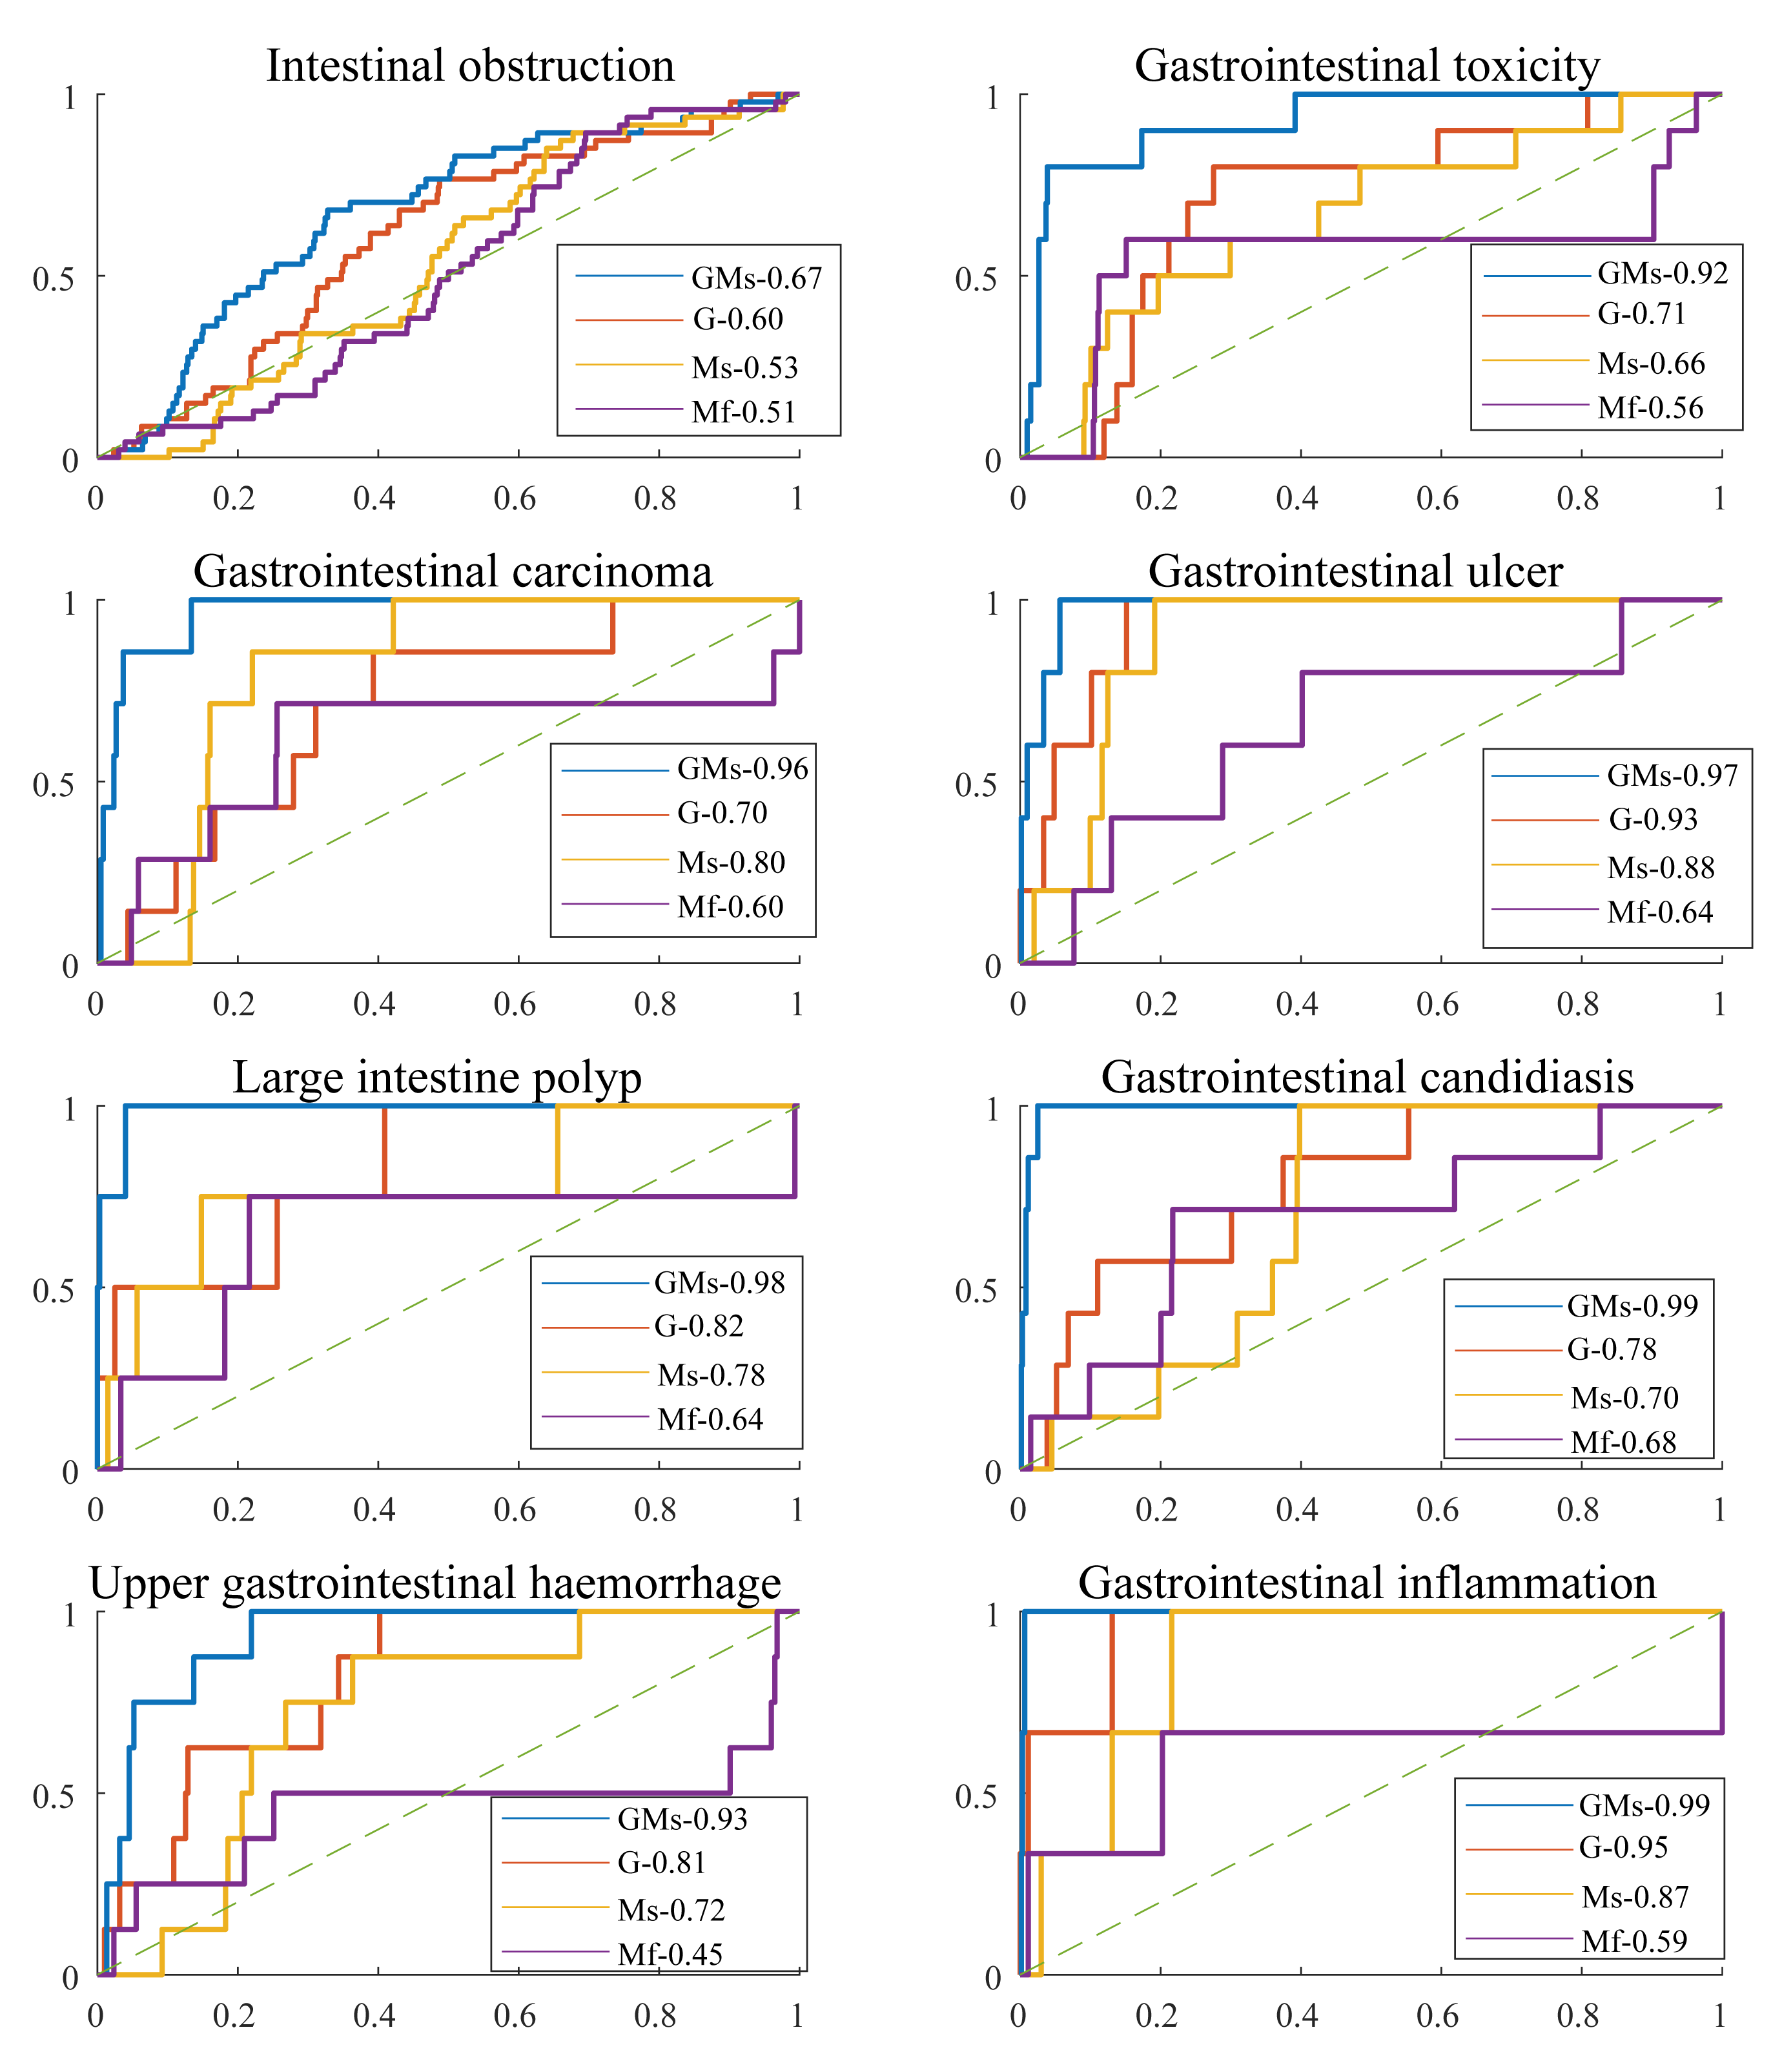
\includegraphics[width=\textwidth,height=\textheight,keepaspectratio]{sideEffects/Figure3.png}%Figure from images\Figure1.png
	\caption[Prediction of individual side effect labels.]{(Continued on the following page.)}
	\label{fig:seff3}
\end{figure}
\begin{figure}[t]
  \contcaption{Out-of-sample ROC curve for intestinal obstruction, gastrointestinal toxicity, carcinoma, ulcer, polyp, candidasis, hemorrhage, and inflammation. The features used for comparison were the sampled flux values in metabolic models, the minimal and maximal flux values per reaction as reported by FVA, gene expression reported in the connectivity map, and the combined gene expression and sampled reaction flux value. The comparison was performed using the area under the ROC curve. G stands for genes, Ms for metabolism sampling, Mf for metabolism FVA, and GMs for genes combined with metabolism sampling.}% Continued caption
\end{figure}
\section{Discussion}
The prediction of side effects using only \textit{in vitro} data of small molecules is a requisite of safe first-in-human trials and low attrition rates in the clinical phases.  The connectivity map of drug signatures \cite{subramanian2017next} provided a large set of gene expression profiles corresponding to small molecules perturbagens. Therefore, we modelled the metabolism of gut wall under drug-induced perturbation to predict iatrogenic effects using an SVM classifier. Sampling of the metabolic model provided better classification results than FVA bounds as features. Moreover, combining gene expression with modelling captured both metabolic and non-metabolic effects in relation to side effect development. Finally, classifying compounds with respect to their metabolic and transcriptomic fingerprint suggested drug repurposing strategies that could provide new therapeutic alternatives.
\subsection{Model generation and parameter selection}
\begin{figure}[!htp]
\centering
	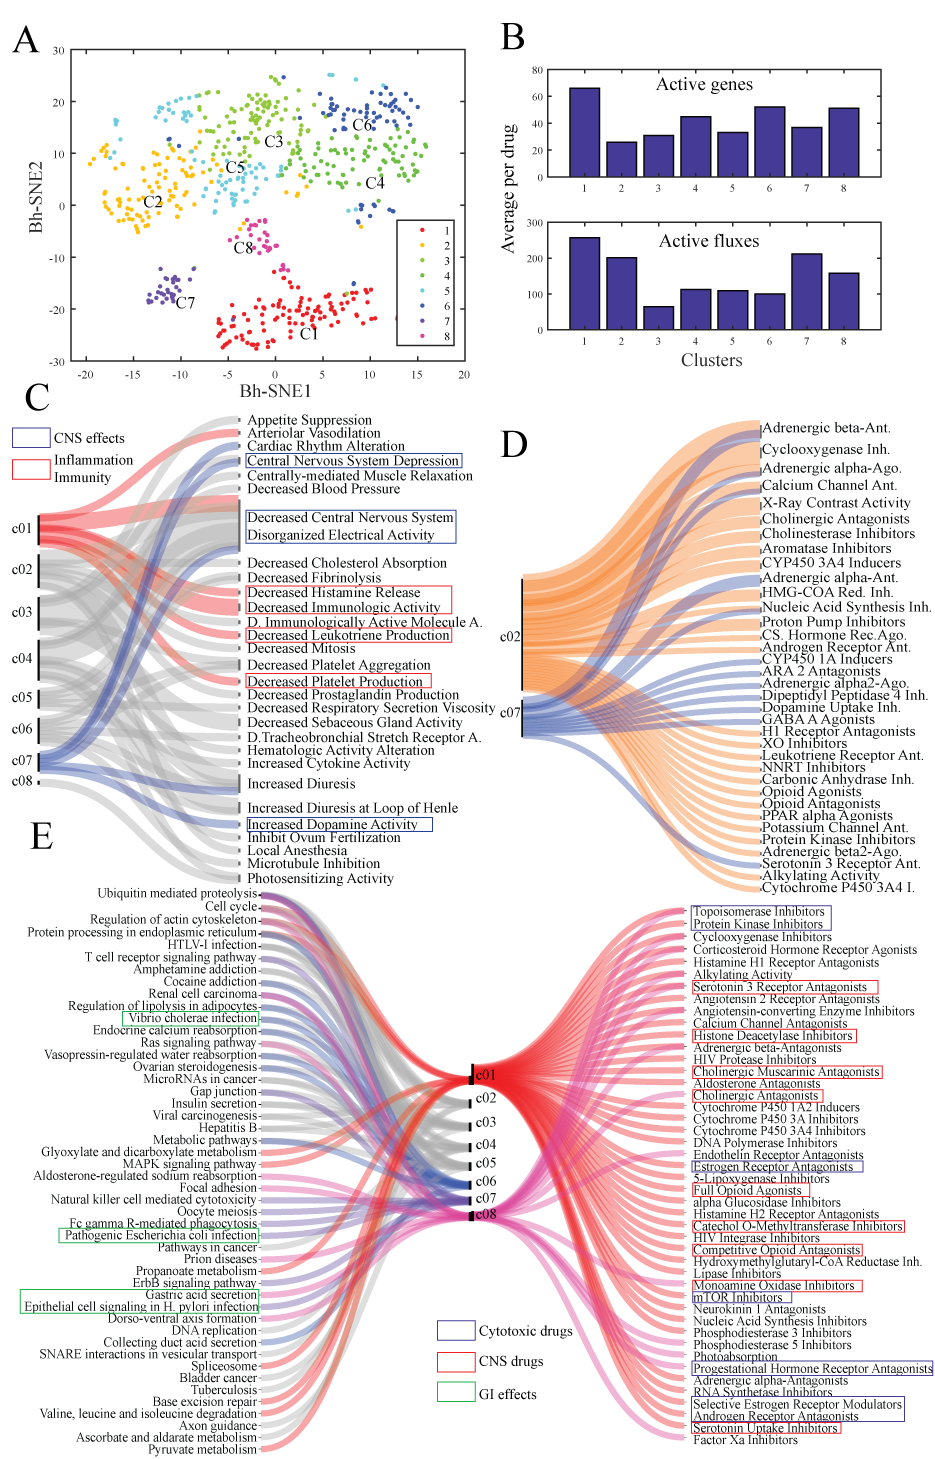
\includegraphics[width=\textwidth,height=\textheight,keepaspectratio]{sideEffects/Figure4.png}%Figure from images\Figure1.png
	\caption[Drug community detection.]{(Continued on the following page.)}
	\label{fig:seff4}
\end{figure}
\begin{figure}[t]
  \contcaption{Drug community identification based on measured transcriptional and simulated gut wall metabolic profile. A-Visualisation of the eight validated drug clusters through Barnes-Hut Stochastic Neighbourhood Embedding (Bh-SNE) plot. B-Transcriptional and gut metabolic activity of the identified clusters showed different levels of drug specificity per cluster. C-Bipartite graph of drug clusters and FDA NDCD's physiological effect (PE). D-Bipartite graph of drug clusters and FDA NDCD’s established physiological class (EPC). E-Graph linking drug clusters to FDA NDCD’s mechanism of action (MoA) and KEGG enriched pathways of the gene pertaining to each cluster. The diagram was done using Rawgraphs \cite{Mauri:2017:RVP:3125571.3125585}.}% Continued caption
\end{figure}
The connectivity map \cite{subramanian2017next} provided a large-scale resource of small molecule transcriptomic signature and enabled the genome-wide assessment of drug off-target effects, thereby expanding pharmacology beyond the study of the drug primary target alone. The integration of drug-induced gene expression with generic metabolic models of human metabolism allowed to identify key disrupted metabolic functions \cite{zielinski2015pharmacogenomic} resulting from adverse reactions. Similarly, the integration of known target effects of drugs as identified from DrugBank \cite{wishart2017drugbank}, and using flux bounds obtained by FVA as features to predict side effects \cite{shaked2016metabolic} allowed to accurately predict several classes of side effects. Although, this approach remains limited to drugs with inhibitory effects on metabolic targets, and \textit{a fortiori} of known targets. In our approach, the integration of drug-induced gene expression with metabolic networks allowed to circumvent the inhibitory target limitation \cite{sahoo2015modeling} and allowed most importantly to model the drug off-target effects which were suggested to be the main driver of side effects. We showed that informing the classifier with the distribution of metabolic fluxes per reaction using sampling rather than providing the bounds of the reaction using flux variability analysis increased the predictive power of the classifier (Figure \ref{fig:seff2}-A,B). Additionally, restricting the prediction to a set of organ-specific side effects using a manually curated tissue-specific metabolic model captured local metabolism in relation to the emergence of organ-specific adverse reactions.\\
Improving the prediction of occurrence of side effects relies greatly on the quality and completeness of the dataset used. It is highly likely that weighting the variables by the side effects frequency per drug can improve the predictions and leverage the prediction of rare side effects. Nevertheless, only 46\% of side effects had frequency information associated whose inclusion did not improve the prediction accuracy (Figure \ref{fig:s6seff}). The missing information could be potentially filled by either manual expert curation or crossing databases. Moreover, the physiological effect and mechanism of action in the FDA NDCD were missing for a number of drugs as well. 
Additionally, the chronopharmacology of drug action is also of paramount importance in detecting the emergence of side effects. The connectivity map provides a number of experiments at several time interval that we did not exploit in our analysis as not all drug-induced gene expression were measured for different time points. Such data can take the predictions from looking at snapshots of transcription and metabolism to dynamical models linking the emergence of  side effects to time-dependant processes.
\subsection{Sampling the metabolic model of the gut wall achieved the highest prediction accuracy}
Conceptually, drug-induced gene expression could play a major role in the genesis of adverse reactions. Particularly, it was shown to be predictive towards side effects classification, especially when combined with other drug features such as chemical structure and cell morphology after treatment \cite{wang2016drug}. The combination of gastrointestinal local metabolism constrained by metabolic gene expression and the differential expression of non-metabolic genes allowed to achieve the most accurate prediction of gastrointestinal side effects (Figure \ref{fig:seff2}-A,B). The combination of multiple layers of biology consisting of transcriptomic and predicted metabolic features was key in capturing drug-induced perturbations related to side effects. Furthermore, the approach can be scaled to several tissues to include all the label of side effects using semi-automatic and manually curated models of human metabolism \cite{schultz2016reconstruction}. Remarkably, sampling metabolic models alone achieved a good accuracy taking into account that only the metabolic subset of genes from the connectivity map was modelled. Therefore, we suggest that a reduced set of \textit{in vitro} experiments to measure the differential expression of metabolic genes would give an invaluable insight into the emergence of adverse reactions of a new chemical entity in the preclinical phase which can guide the rational design of first-in-human trials. Furthermore, the emergence of whole-cell models \cite{karr2012whole,szigeti2017blueprint} that integrate metabolism alongside several physiological functions would allow the mapping of non-metabolic genes onto computational models of the cell to capture the cell-wide disruption of physiological processes that lead to the emergence of side effects. With the generated combined gene and gut wall metabolism matrix in hand, we classified the small molecules with respect to their signatures to highlight their common features.
\subsection{Drug reclassification beyond the chemical class}
Drugs are often classified with respect to their pharmacological indication and their chemical family. The many examples of marketed drug repurposed for new indications \cite{li2015survey} shows that a small molecule can have rather many effects. Drug repurposing have gained great interest in the recent years, as it allows to greatly decrease the drug development process using compounds whose safety is well documented.  
In order to find common properties of drugs, we identified clusters of compounds that share similar genetic and metabolic signatures in the gut wall. Interestingly, compounds that involved a high number of metabolic reactions with a high amplitude of variation included CNS drugs like serotonin antagonists indicated for psychotic episodes that were later suggested to treat chemotherapy-induced emesis. Moreover, those compounds belonged to the same cluster with neurokinin inhibitors that are primarily indicated for the prevention of emesis as well. Serotonin antagonists are also indicated to treat the inflammatory bowel syndrome, which further showed the similarity between the blood brain barrier and the gut wall metabolism and gene expression. Furthermore, anticancer drugs and the drugs that treat their side effects, the anti-emesis drugs, clustered together in the high transcriptomic, high metabolic activity cluster, further supporting the idea that reversing the molecular fingerprint of a compound can reverse its effects. Particularly, reversing the fingerprint of the compound locally, in the gut wall, would be a potential strategy to reverse gastrointestinal side effects of drugs through the administration of co-drugs, while preserving its main activity in the target tissue.\\
Furthermore, the clusters of drugs that we identified in our analysis did not match FDA marketing date (Figure \ref{fig:s9seff}-B). Despite the emergence of the key-lock paradigm \cite{medina2013shifting} in drug development using molecular dynamics and docking experiments in early 1990s that decreased the number of drugs interacting with a high number of targets, colloquially  called 'dirty drugs', there are still opportunities for further enhancement in the design of precise therapies. \\
We developed and employed a multi-label support vector machine on genetic and metabolic fingerprint of marketed small molecule compounds to accurately predict the occurrence of gastrointestinal side effects. The drug features allowed to classify drugs based on their metabolic and genetic profile, which is a promising avenue for drug repurposing to revert side effects and unravel new indications. The development of large scale, publicly available, compound resources combined with complex mathematical models of cellular biology provides a new way of providing patients with safer and more effective therapies.
\subsection*{Acknowledgements}
The authors would like to acknowledge Dr. Peter Banda at the Luxembourg Centre for Systems Biomedicine (LCSB) for the helpful discussions and the important suggestions on the work as well as the Molecular Systems Physiology lab members at the LCSB for insightful comments on the manuscript and in particular Alberto Noronha for technical assistance. 
